\chapter{Resultados}
En este capítulo se presentan los resultados definitivos obtenidos tras la fase de desarrollo e integración de la plataforma \textit{SkiClubManager}. Las vistas del sistema se exponen organizadas de acuerdo con la modularidad de su arquitectura en el \textit{frontend}, la cual segmenta la lógica en un espacio común de autenticación y tres perfiles operacionales específicos.

Para evitar la redundancia documental, aquellas interfaces funcionales del cuerpo técnico que comparten un diseño análogo entre los perfiles de entrenador y administrador se describen de forma unificada, haciendo hincapié en las capacidades de control exclusivas de la administración.

\section{Módulo de acceso común}
El punto de entrada del sistema agrupa los componentes de control y seguridad iniciales implementados en el directorio \texttt{comun} (Figura \ref{fig:inicio}).

Estas interfaces gestionan el ciclo inicial de los JSON Web Tokens (JWT) y el flujo de recuperación de credenciales:
\begin{itemize}
    \item \textbf{Pantalla de Login:} Interfaz limpia que captura las credenciales del usuario, interactúa con el \textit{backend} en Node.js para validar los roles y almacena el token de sesión de forma segura.
    \item \textbf{Pantalla de Registro de Padres:} Componente encargado del alta de nuevos tutores en el sistema. Captura los datos personales y de contacto necesarios para la gestión administrativa del club, vinculando opcionalmente el perfil del padre con los registros de los deportistas a su cargo para delimitar el acceso posterior a los módulos de asistencia y progreso.
    \item \textbf{Recuperación y Cambio de Claves:} Componentes dedicados a la gestión autónoma de la seguridad por parte del usuario, habilitando el restablecimiento de contraseñas comprometidas u olvidadas.
\end{itemize}

\begin{figure}[htbp]
    \centering
    \begin{subfigure}[b]{0.31\textwidth}
        \centering
        
\includegraphics[width=\textwidth]{imagenes/inicio.png}
        \caption{Pantalla de inicio.}
        \label{fig:inicio}
    \end{subfigure}
    \hfill
    \begin{subfigure}[b]{0.31\textwidth}
        \centering
        
\includegraphics[width=\textwidth]{imagenes/solicitud_registro_1.png}
        \caption{Registro (Datos Tutor).}
        \label{fig:registroTutor}
    \end{subfigure}
    \hfill
    \begin{subfigure}[b]{0.31\textwidth}
        \centering
        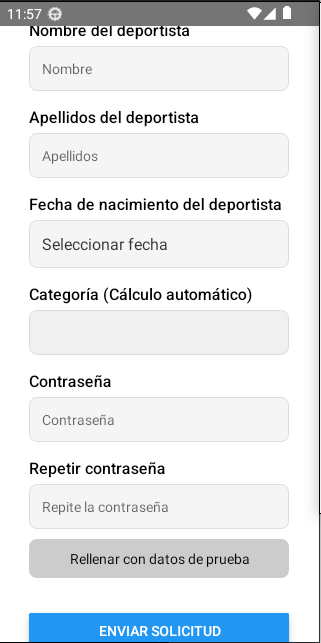
\includegraphics[width=\textwidth]{imagenes/solicitud_registro_2.png}
        \caption{Registro (Datos Tutor 2).}
        \label{fig:registroTutor2}
    \end{subfigure}
    
    \caption{Interfaces correspondientes a la pantalla de bienvenida y al formulario secuencial de alta para nuevos tutores y deportistas.}
    \label{fig:flujo_registro_completo}
\end{figure}

\subsubsection{Proceso de Alta y Registro de Nuevos Tutores}

Para los usuarios con el rol de padre que acceden por primera vez a la plataforma, el sistema requiere la cumplimentación de un formulario secuencial estructurado en dos bloques lógicos, facilitando la recolección de datos y la posterior vinculación jerárquica con el deportista a su cargo.

En la primera fase, ilustrada en la Figura~\ref{fig:registroTutor} y ~\ref{fig:registroTutor2}, el solicitante introduce sus datos personales. El correo electrónico actúa como identificador único en el sistema, sirviendo posteriormente para la autenticación mediante JWT y los flujos de recuperación de credenciales.

Finalmente, al pulsar el botón de envío, los datos se mandan al servidor para su verificación. Tras comprobar que la información es correcta y proteger la contraseña, el sistema almacena de forma ordenada el perfil del padre y del deportista, enlazándolos directamente.

\begin{figure}[htbp]
    \centering
    % ========== PRIMERA FILA (Las dos primeras pantallas) ==========
    \begin{subfigure}[t]{0.3\textwidth}
        \centering
        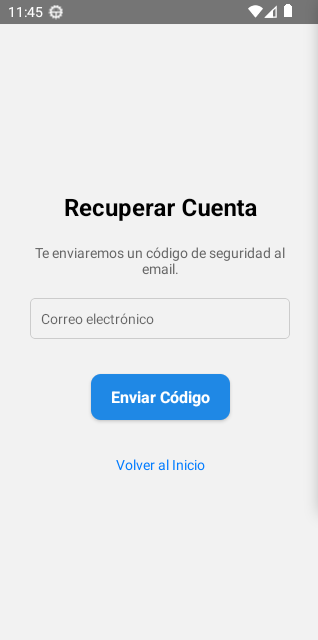
\includegraphics[width=\textwidth]{imagenes/recuperarContraseña.png}
        \caption{Solicitud de recuperación.}
        \label{fig:recuperarContrasena}
    \end{subfigure}
    \hfill
    \begin{subfigure}[t]{0.3\textwidth}
        \centering
        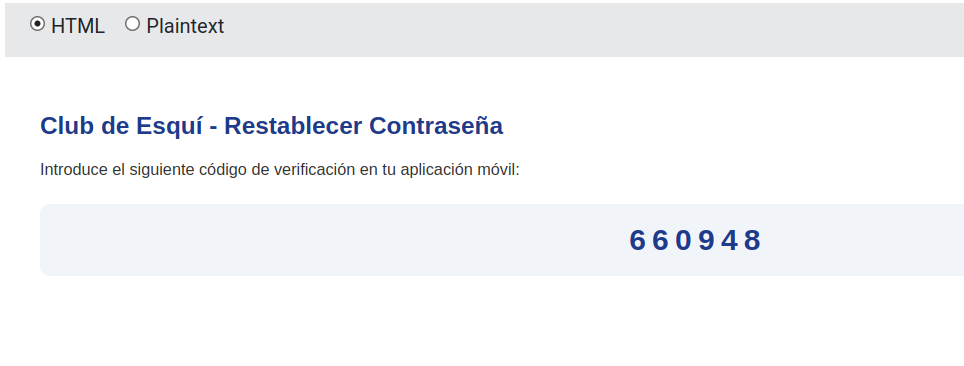
\includegraphics[width=\textwidth]{imagenes/codigo_restablecer.png}
        \caption{Código de validación.}
        \label{fig:codigoRestablecer}
    \end{subfigure}

    \vspace{0.5cm} % Espacio de separación vertical entre filas

    % ========== SEGUNDA FILA (Las dos últimas pantallas) ==========
    \begin{subfigure}[t]{0.3\textwidth}
        \centering
        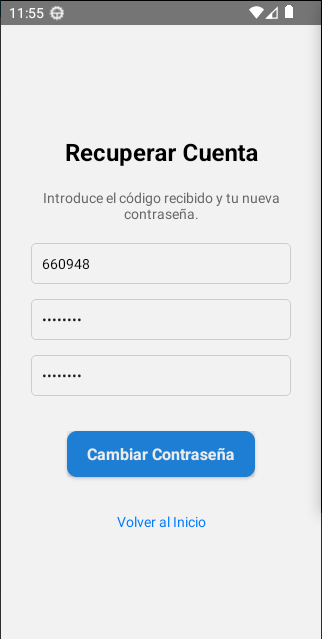
\includegraphics[width=\textwidth]{imagenes/recuperar_contraseña_relleno.png}
        \caption{Formulario completado.}
        \label{fig:recuperarRelleno}
    \end{subfigure}
    \hfill
    \begin{subfigure}[t]{0.3\textwidth}
        \centering
        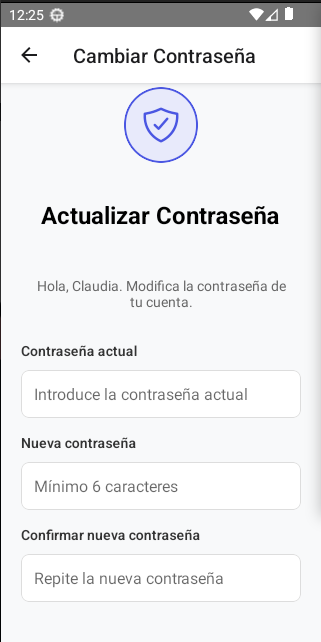
\includegraphics[width=\textwidth]{imagenes/cambiar_contraseña.png}
        \caption{Formulario para cambiar contraseña.}
        \label{fig:cambiarContrasena}
    \end{subfigure}
    
    \caption{Interfaces correspondientes al flujo completo de validación de seguridad, restablecimiento y cambio autónomo de credenciales de usuario.}
    \label{fig:grupo_restablecimiento_completo}
\end{figure}

\newpage
\subsubsection{Flujo de Recuperación de Contraseña}

El sistema dispone de un flujo seguro y automatizado para el restablecimiento de credenciales de los usuarios de la plataforma, el cual interactúa directamente con la API REST y la base de datos del club.

El proceso comienza en la interfaz de inicio de sesión de la aplicación móvil, englobada en el bloque de autenticación de la Figura~\ref{fig:recuperarContrasena}. Al solicitar la recuperación, el usuario introduce su dirección de correo electrónico. El backend en Node.js recibe la petición, valida la existencia del perfil en la base de datos MySQL y genera un token de seguridad temporal que se envía automáticamente al buzón del solicitante.

Tras recibir dicha clave efímera, el usuario la introduce en la pantalla de validación intermedia que se detalla en la Figura~\ref{fig:codigoRestablecer}. Este paso intermedio permite al servidor comprobar que el solicitante posee acceso legítimo a la cuenta de correo vinculada al deportista o entrenador.

Una vez validado el código en el servidor, la aplicación habilita la transición al formulario definitivo, ilustrado en la Figura~\ref{fig:recuperarRelleno}. En esta interfaz, el usuario introduce y confirma su nueva contraseña. Al procesar el formulario, estos datos se envían de forma segura al sistema para registrar la nueva clave de acceso, guardando los cambios de inmediato y restableciendo por completo el acceso protegido a la aplicación.

\section{Desglose de Interfaces y Resultados por Rol}
\label{sec:interfaces_roles}

En esta sección se exponen los resultados visuales y funcionales definitivos de la aplicación, organizados de forma estricta según el perfil del usuario autenticado. Esta estructura permite evaluar de manera independiente los flujos de trabajo, las restricciones de acceso y las interfaces maquetadas en React Native para cada uno de los roles operativos del sistema.

\subsection{Perfil del Entrenador}
\label{subsec:rol_entrenador}
El perfil del entrenador está diseñado para que el entrenador solo vea aquellos entrenamientos y deportistas de su categoría, a excepción del calendario que permite una visualización global de todos los eventos. Sus pantallas principales, localizadas en el directorio \texttt{entrenador} son las siguientes:

\noindent \textbf{Panel Inicial del Entrenador:} Pantalla de inicio que se despliega inmediatamente al acceder a la aplicación. Actúa como un cuadro de mando unificado que ofrece accesos directos a las herramientas clave del día a día (como la agenda o la galería multimedia) y destaca en primer plano las próximas sesiones programadas para el grupo de deportistas a su cargo. \par \smallskip
\begin{figure}[htbp]
    \centering
    \begin{subfigure}[t]{0.3\textwidth}
        \centering
        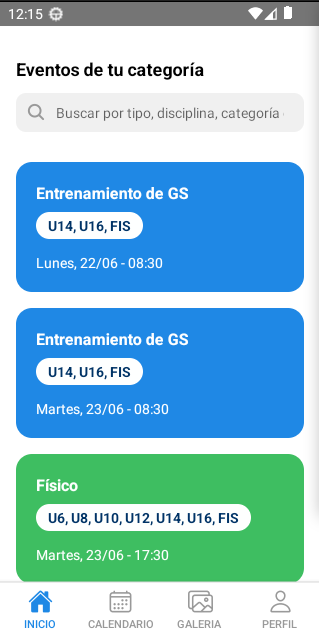
\includegraphics[width=\textwidth]{imagenes/inicio_entrenador.png}
        \caption{Pantalla de inicio del entrenador.}
        \label{fig:inicioEntrenador}
    \end{subfigure}
    \hfill
    \begin{subfigure}[t]{0.3\textwidth}
        \centering
        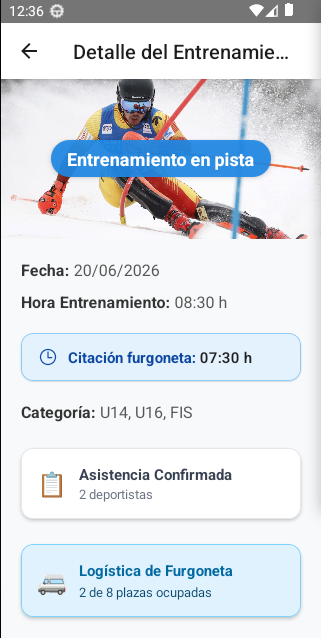
\includegraphics[width=\textwidth]{imagenes/detalle_entreno.png}
        \caption{Vista de detalles de la sesión.}
        \label{fig:detalleEntreno}
    \end{subfigure}
    
    \caption{Interfaces operativas del perfil técnico: panel principal de bienvenida (a) y desglose detallado tras la selección de una actividad (b).}
    \label{fig:flujo_inicio_detalle_entrenador}
\end{figure}

\begin{figure}[htbp]
    \centering
    \begin{subfigure}[t]{0.3\textwidth}
        \centering
        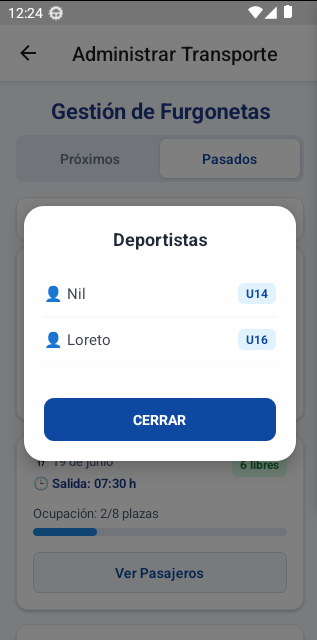
\includegraphics[width=\textwidth]{imagenes/lista_transporte.png}
        \caption{Ventana de pasajeros de la furgoneta.}
        \label{fig:listaTransporteModal}
    \end{subfigure}
    \hfill
    \begin{subfigure}[t]{0.3\textwidth}
        \centering
        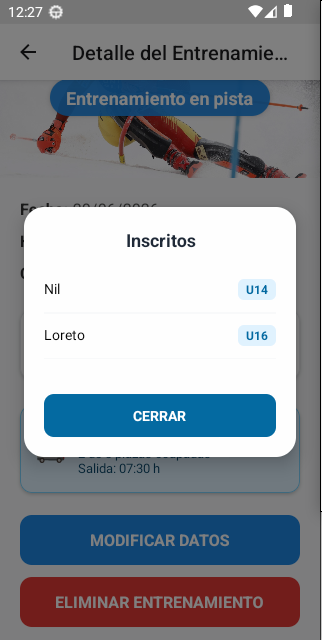
\includegraphics[width=\textwidth]{imagenes/detalle_inscritos.png}
        \caption{Ventana de deportistas inscritos.}
        \label{fig:detalleInscritosModal}
    \end{subfigure}
    
    \caption{Interfaces de las ventanas emergentes de consulta detallada: listado de pasajeros asignados al transporte (a) y desglose de corredores inscritos en la sesión técnica (b).}
    \label{fig:grupo_modals_operativos}
\end{figure}

\newpage

\begin{itemize}
    \item \textbf{Panel Principal del Entrenador (Figura~\ref{fig:inicioEntrenador}):} Es la pantalla de bienvenida que se muestra al iniciar sesión. Actúa como un cuadro de mando que ofrece un acceso directo y rápido a las herramientas clave, como el calendario completo y la galería de vídeos. Además, destaca las próximas citas programadas en la agenda del día de forma directa para facilitar la organización en la nieve.
    
    \item \textbf{Desglose y Detalles de la Sesión (Figura~\ref{fig:detalleEntreno}):} Al presionar sobre cualquiera de los entrenamientos que aparecen en el panel de inicio o en el calendario, la aplicación redirige al usuario a esta interfaz. En ella se detalla minuciosamente la planificación de la jornada: el horario del entrenamiento, la disciplina de entrenamiento (como gigante, supergigante o eslalon), la furgoneta asignada y el listado de deportistas convocados, sirviendo como paso previo indispensable antes de tramitar la asistencia.
    
    \item \textbf{Listado de Pasajeros de Furgoneta (Figura~\ref{fig:listaTransporteModal}):} Ventana emergente interactiva vinculada al módulo de logística de transportes colectivos. Al accionar el botón de consulta de pasajeros, el sistema despliega este componente superpuesto que extrae en tiempo real las asignaciones de asientos, listando con nombre y categoría a los deportistas que tienen reservada su plaza para ese trayecto específico hacia la estación invernal. \par \smallskip

    \item \textbf{Consulta de Deportistas Inscritos (Figura~\ref{fig:detalleInscritosModal}):} Componente modal integrado dentro de la vista general de detalles de la actividad. Ofrece al cuerpo técnico una ventana rápida de supervisión para comprobar la nómina exacta de corredores confirmados para la sesión de entrenamiento. Clasifica automáticamente a los atletas según su categoría de edad competitiva, permitiendo al preparador dimensionar los recursos técnicos y el material de trazado antes de iniciar la jornada en la nieve.
\end{itemize}

\noindent \textbf{Calendario del Entrenador:} Interfaz principal del técnico que muestra la planificación mensual de entrenamientos mediante el código de colores semánticos (nieve, físico o competición). Permite acceder al detalle de cada sesión.
\begin{figure}[htbp]
    \centering
    % ========== FILA 1: CALENDARIO (Las 2 imágenes que van primero) ==========
    \begin{subfigure}[t]{0.25\textwidth}
        \centering
        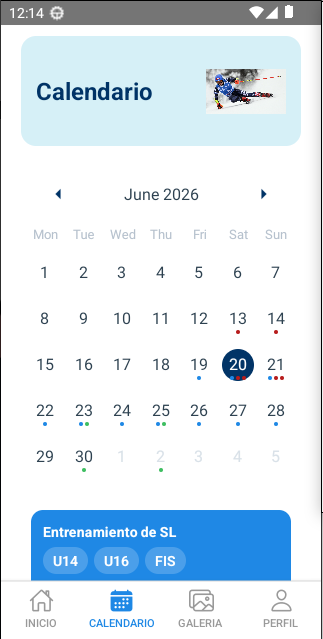
\includegraphics[width=\textwidth]{imagenes/calendario_1.png}
        \caption{Vista mensual.}
        \label{fig:calendario1}
    \end{subfigure}
    \hspace{1cm} % Espaciado horizontal para centrar las dos imágenes
    \begin{subfigure}[t]{0.25\textwidth}
        \centering
        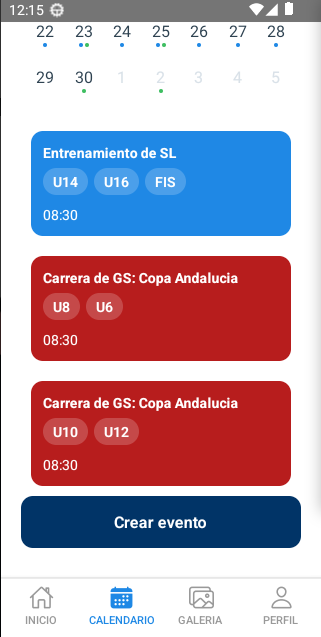
\includegraphics[width=\textwidth]{imagenes/calendario_2.png}
        \caption{Eventos diarios.}
        \label{fig:calendario2}
    \end{subfigure}

    \vspace{0.5cm} % Separación entre bloques

    % ========== FILA 2: CREACIÓN - PARTE 1 (3 imágenes del asistente) ==========
    \begin{subfigure}[t]{0.25\textwidth}
        \centering
        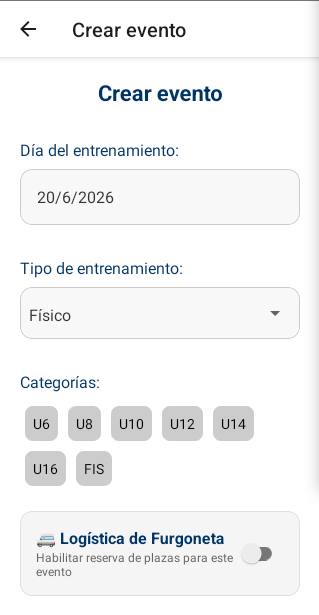
\includegraphics[width=\textwidth]{imagenes/crear_evento_1.png}
        \caption{Datos iniciales y logística.}
        \label{fig:crear_evento_1}
    \end{subfigure}
    \hfill
    \begin{subfigure}[t]{0.25\textwidth}
        \centering
        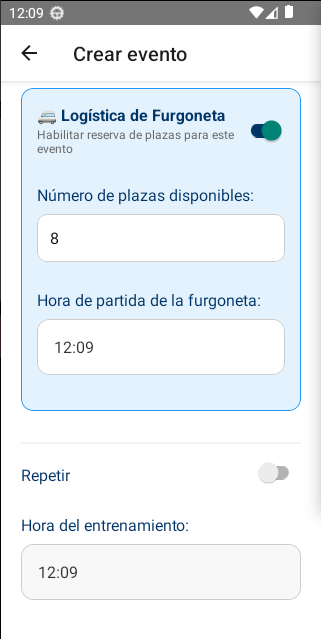
\includegraphics[width=\textwidth]{imagenes/crear_evento_2.png}
        \caption{Horarios y transporte.}
        \label{fig:crear_evento_2}
    \end{subfigure}
    \hfill
    \begin{subfigure}[t]{0.25\textwidth}
        \centering
        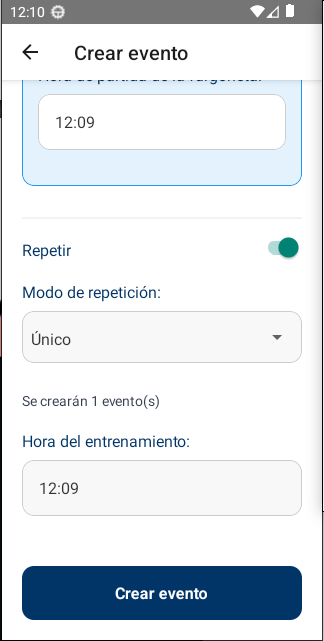
\includegraphics[width=\textwidth]{imagenes/crear_evento_unico.png}
        \caption{Programación única.}
        \label{fig:crear_evento_unico}
    \end{subfigure}

    \vspace{0.4cm} % Separación entre subfilas del asistente

    % ========== FILA 3: CREACIÓN - PARTE 2 (Las 2 imágenes restantes) ==========
    \begin{subfigure}[t]{0.25\textwidth}
        \centering
        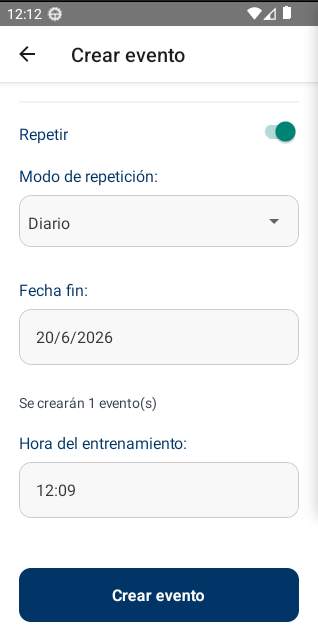
\includegraphics[width=\textwidth]{imagenes/crear_evento_diario.png}
        \caption{Programación diaria.}
        \label{fig:crear_evento_diario}
    \end{subfigure}
    \hspace{0.5cm} % Espacio centrado para la última fila
    \begin{subfigure}[t]{0.25\textwidth}
        \centering
        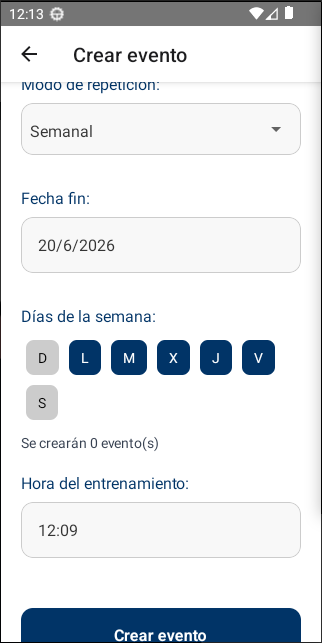
\includegraphics[width=\textwidth]{imagenes/crear_evento_semanal.png}
        \caption{Programación semanal.}
        \label{fig:crear_evento_semanal}
    \end{subfigure}
    
    \caption{Interfaces del módulo de planificación: vistas de la agenda (a, b) y pasos del asistente para la creación de entrenamientos según la modalidad (c, d, e, f, g).}
    \label{fig:planificacion_y_creacion_completa}
\end{figure}

\newpage
\begin{itemize}
    \item \textbf{Evento Único (Figura~\ref{fig:crear_evento_unico}):} Esta modalidad está diseñada para registrar actividades puntuales y aisladas en el calendario del club. Se utiliza principalmente para convocar eventos extraordinarios que no se repiten en el tiempo, como una carrera o un entrenamiento técnico especial en una fecha concreta. Al programarlo, el sistema genera una única cita en la agenda de los usuarios afectados.
    
    \item \textbf{Programación Diaria (Figura~\ref{fig:crear_evento_diario}):} Esta opción está pensada para planificar bloques de entrenamientos intensivos que se llevan a cabo de forma consecutiva durante varios días seguidos. Es la herramienta ideal para organizar campus vacacionales, como los tradicionales entrenamientos de Navidad, Reyes o Semana Santa, así como las concentraciones de pretemporada fuera de la estación habitual. El asistente permite fijar un rango de fechas y replica automáticamente la actividad en jornadas consecutivas con un solo envío.
    
    \item \textbf{Programación Semanal (Figura~\ref{fig:crear_evento_semanal}):} Pensada para estructurar la rutina y la planificación a largo plazo de la temporada. Se utiliza para automatizar todas aquellas sesiones que se repiten de forma fija los mismos días de la semana. El entrenador simplemente selecciona los días correspondientes y el sistema automatiza las convocatorias para todo el periodo establecido.
\end{itemize}

\noindent \textbf{Creación y Modificación de Eventos}: Formularios dedicados a la gestión de la agenda. Permiten al entrenador reajustar los horarios de forma dinámica ante imprevistos meteorológicos en alta montaña.

\begin{figure}[htbp]
    \centering
    \begin{subfigure}[t]{0.28\textwidth}
        \centering
        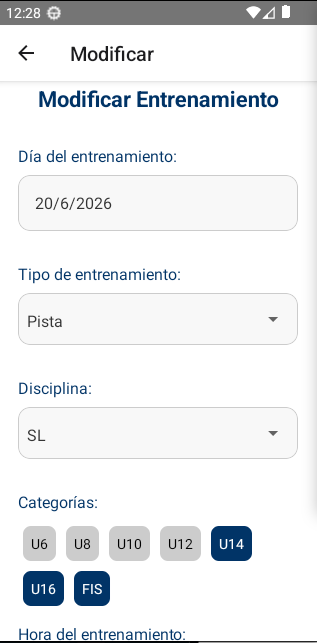
\includegraphics[width=\textwidth]{imagenes/modificar_enrteno.png}
        \caption{Modificación de datos básicos.}
        \label{fig:modificarEntreno1}
    \end{subfigure}
    \hfill
    \begin{subfigure}[t]{0.28\textwidth}
        \centering
        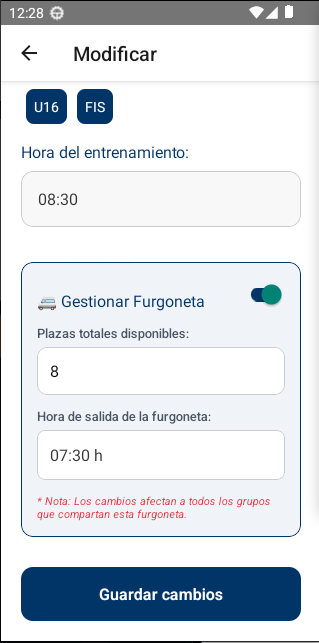
\includegraphics[width=\textwidth]{imagenes/modificar_entreno_2.png}
        \caption{Ajuste logístico y horarios.}
        \label{fig:modificarEntreno2}
    \end{subfigure}
    \hfill
    \begin{subfigure}[t]{0.28\textwidth}
        \centering
        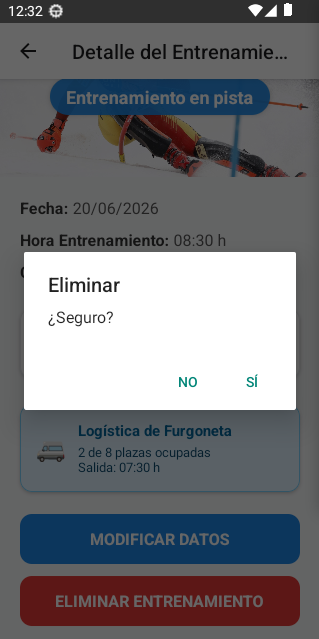
\includegraphics[width=\textwidth]{imagenes/eliminar_entreno.png}
        \caption{Confirmación de eliminación.}
        \label{fig:eliminarEntreno}
    \end{subfigure}
    
    \caption{Interfaces del proceso de edición de parámetros en tiempo real y cancelación de sesiones de entrenamiento programadas.}
    \label{fig:flujo_modificar_eliminar}
\end{figure}


\begin{itemize}
    \item \textbf{Modificación de Datos Básicos (Figura~\ref{fig:modificarEntreno1}):} Permite al entrenador alterar los parámetros iniciales de una actividad ya publicada, como el tipo de entrenamiento, la estación invernal elegida o reasignar las categorías de los deportistas convocados si se decide unificar grupos de trabajo.
    
    \item \textbf{Ajuste Logístico y Horarios (Figura~\ref{fig:modificarEntreno2}):} Enfocado a cambiar las franjas horarias de la sesión o reorganizar la asignación de plazas en las furgonetas de transporte del club. Esta pantalla es fundamental en el día a día del club para mitigar imprevistos meteorológicos en alta montaña (como ráfagas de viento fuertes o congelación de remontes) sin necesidad de rehacer la convocatoria desde cero.
    
    \item \textbf{Confirmación de Eliminación (Figura~\ref{fig:eliminarEntreno}):} Un asistente de seguridad que se despliega al intentar cancelar una sesión. Muestra de forma muy clara los detalles del evento que se va a borrar y solicita una confirmación explícita para evitar pérdidas accidentales de datos en el historial de la temporada.
\end{itemize}

\newpage

\noindent \textbf{Galería del Entrenador:} Repositorio visual donde el entrenador captura o sube imágenes de los entrenamientos, indexándolas por fecha y categoría para el posterior video-análisis biomecánico de los virajes.

\begin{figure}[htbp]
    \centering
    % ========== PRIMERA FILA (Subida y Paneles) ==========
    \begin{subfigure}[t]{0.3\textwidth}
        \centering
        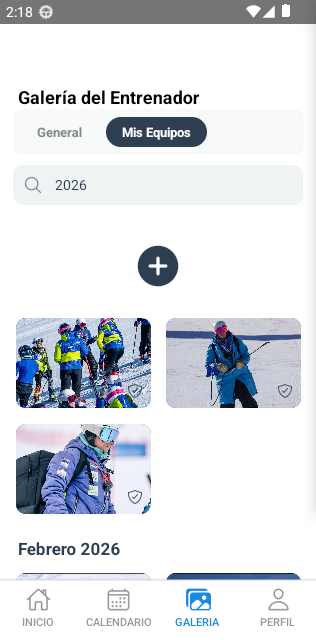
\includegraphics[width=\textwidth]{imagenes/galeria_entrenador.png}
        \caption{Galería del entrenador.}
        \label{fig:galeriaAdminPanel}
    \end{subfigure}
    \hfill
    \begin{subfigure}[t]{0.3\textwidth}
        \centering
        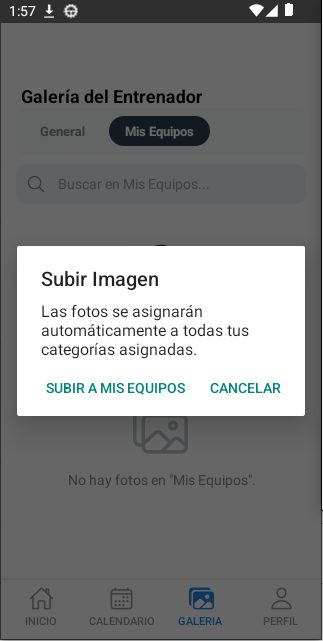
\includegraphics[width=\textwidth]{imagenes/subir_galeria.png}
        \caption{Ventana de confirmación de subida.}
        \label{fig:subirGaleriaModal}
    \end{subfigure}

    \vspace{0.5cm}

    % ========== SEGUNDA FILA (Carrete y Borrado) ==========
    \begin{subfigure}[t]{0.3\textwidth}
        \centering
        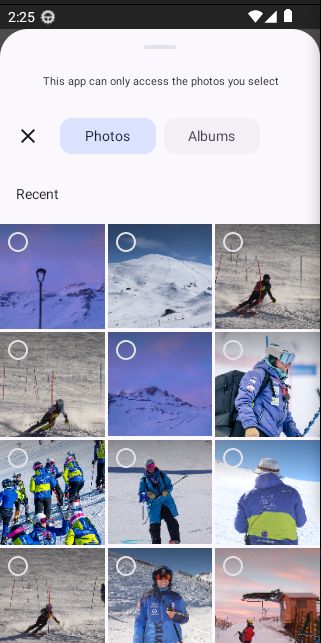
\includegraphics[width=\textwidth]{imagenes/subir_fotos_galeria_drive.png}
        \caption{Acceso al almacenamiento local.}
        \label{fig:subirFotosDriveCarrete}
    \end{subfigure}
    \hfill
    \begin{subfigure}[t]{0.3\textwidth}
        \centering
        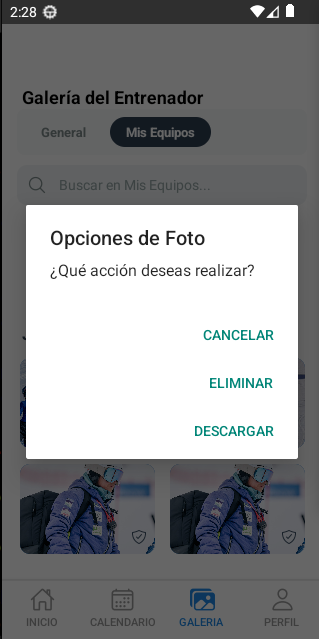
\includegraphics[width=\textwidth]{imagenes/eliminar_galeria_entrenador.png}
        \caption{Menú contextual de opciones.}
        \label{fig:eliminarGaleriaEntrenador}
    \end{subfigure}
    
    \caption{Interfaces del módulo multimedia: flujo guiado de carga asíncrona de archivos (b, c), visualización por categorías competitivas (a) y herramientas de depuración de almacenamiento (d).}
    \label{fig:cuadridula_galeria_multimedia}
\end{figure}

\noindent \textbf{Asistente de Carga Multimedia:} Flujo guiado que permite a los usuarios autorizados incorporar nuevo material gráfico obtenido durante las bajadas en la pista. El sistema interactúa de manera nativa con la API de selección de archivos del sistema operativo móvil para abrir el carrete del dispositivo. Al seleccionar los elementos, se despliega una ventana emergente de confirmación que indexa automáticamente los recursos, asignándolos de forma simultánea a todas las categorías competitivas que el técnico tenga vinculadas en su perfil de trabajo. \par \smallskip

\noindent \textbf{Panel de Control Multimedia General:} Interfaz centralizada de supervisión que organiza cronológica y lógicamente el repositorio del club. Cuenta con una barra de filtrado rápido segmentada por categorías de edad (desde U6 hasta la categoría FIS) y un motor de búsqueda por texto. Esto permite a los entrenadores y administradores localizar secuencias específicas de vídeo de forma inmediata para llevar a cabo sesiones de video-análisis técnico en la zona de descanso o durante los traslados. \par \smallskip

\noindent \textbf{Administración y Depuración de Almacenamiento:} Menú contextual de seguridad que se activa al interactuar de forma prolongada sobre cualquier miniatura del repositorio. Con el objetivo de optimizar la capacidad del servidor de almacenamiento asíncrono y eliminar tomas descartadas o de baja calidad, esta interfaz ofrece funciones directas de descarga local en alta resolución o borrado definitivo, actualizando el estado de la base de datos de manera inmediata.

\noindent \textbf{Perfil del entrenador:}
\begin{figure}[htbp]
    \centering
    % ========== FILA 1: PERFIL PRINCIPAL ==========
    \begin{subfigure}[t]{0.35\textwidth}
        \centering
        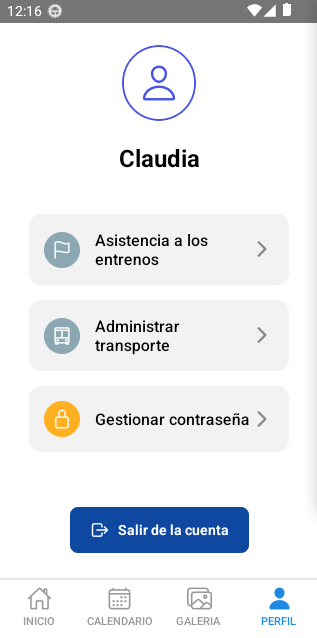
\includegraphics[width=\textwidth]{imagenes/perfil_entrenador.png}
        \caption{Interfaz de perfil del usuario.}
        \label{fig:perfilEntrenador}
    \end{subfigure}

    \vspace{0.4cm}

    % ========== FILA 2: ASISTENCIA (2 imágenes) ==========
    \begin{subfigure}[t]{0.23\textwidth}
        \centering
        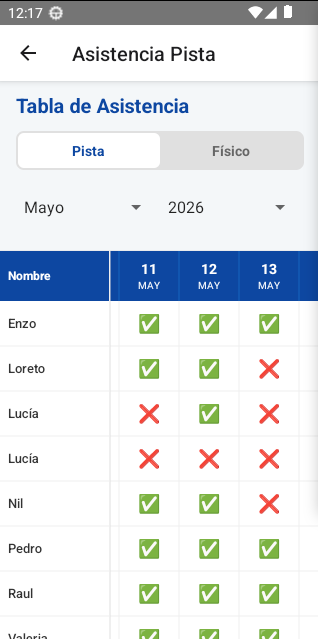
\includegraphics[width=\textwidth]{imagenes/asistencia_pista_entrenador.png}
        \caption{Historial en pista.}
        \label{fig:asistenciaPista2}
    \end{subfigure}
    \hfill
    \begin{subfigure}[t]{0.23\textwidth}
        \centering
        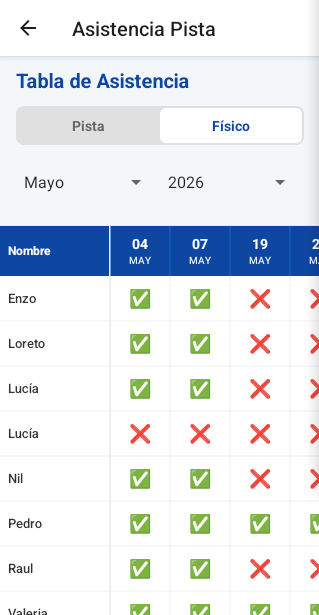
\includegraphics[width=\textwidth]{imagenes/asistencia_fisico_entrenador.png}
        \caption{Historial físico.}
        \label{fig:asistenciaFisico2}
    \end{subfigure}
    \hfill
    % ========== FILA 2: TRANSPORTE (2 imágenes) ==========
    \begin{subfigure}[t]{0.23\textwidth}
        \centering
        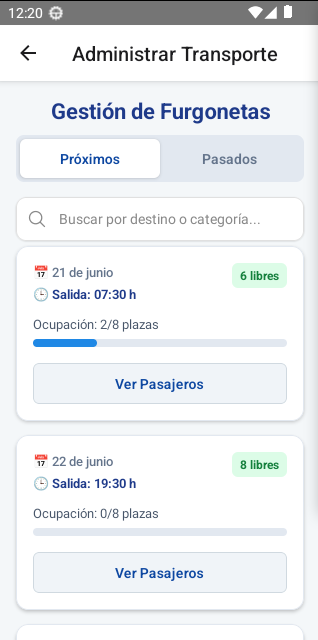
\includegraphics[width=\textwidth]{imagenes/transporte_proximos.png}
        \caption{Rutas próximas.}
        \label{fig:transporteProximos}
    \end{subfigure}
    \hfill
    \begin{subfigure}[t]{0.23\textwidth}
        \centering
        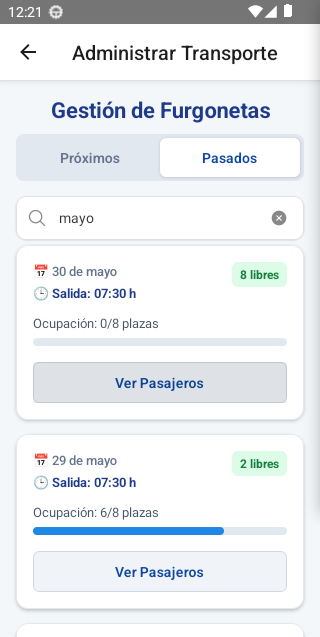
\includegraphics[width=\textwidth]{imagenes/transporte_pasados.png}
        \caption{Rutas pasadas.}
        \label{fig:transportePasados}
    \end{subfigure}
    
    \caption{Interfaces del panel de perfil del entrenador (a) y desglose de sus submódulos de gestión de asistencia (b, c) y control logístico de furgonetas (d, e).}
    \label{fig:flujo_perfil_gestion_entrenador}
\end{figure}

\begin{itemize}
    \item \textbf{Gestión de Perfil del Entrenador (Figura~\ref{fig:perfilEntrenador}):} Actúa como la zona centralizada de configuración para el usuario técnico. Desde este panel, el profesional accede de forma directa a sus históricos consolidados de asistencia, la asignación de transportes para los entrenamientos y las opciones de actualización de credenciales.
    
    \item \textbf{Históricos de Asistencia Cruzada (Figuras~\ref{fig:asistenciaPista2} y~\ref{fig:asistenciaFisico2}):} Pantallas de consulta que permiten al entrenador revisar el histórico de los partes de asistencia ya validados y consolidados en semanas anteriores. la información se divide mediante pestañas interactivas entre las sesiones técnicas sobre la nieve (pista) y el trabajo de acondicionamiento fuera de ella (físico), facilitando la evaluación interna de la constancia de los deportistas.
    
    \item \textbf{Control Centralizado de Furgonetas (Figuras~\ref{fig:transporteProximos} y~\ref{fig:transportePasados}):} Módulo logístico dedicado a la supervisión del transporte colectivo del club. Cuenta con un sistema de filtrado bimodal que segmenta las rutas de recogida planificadas para los días venideros (próximos) y el registro de traslados completados (pasados). Ofrece una lectura visual clara a través de barras de progreso que indican la tasa de ocupación de las plazas en tiempo real y permite listar de manera unificada la hoja de pasajeros convocada para cada trayecto a la estación.

    \item \textbf{Recuperación y Cambio de Contraseña:} Este apartado del perfil redirige al usuario al formulario activo de actualización de claves. El funcionamiento interno del componente, las restricciones de seguridad basadas en tokens temporales y la validación de la contraseña actual frente a la nueva ya han sido detallados rigurosamente al inicio de este capítulo, concretamente en la figura~\ref{fig:cambiarContrasena}.

\end{itemize}

\newpage
\subsection{Perfil del Administrador}
\label{subsec:rol_administrador}
El perfil de administración comparte la lógica de planificación del entrenador, pero añade la gestión de la infraestructura lógica y el censo general del club.
\\
\noindent \textbf{Panel de Control del Administrador:} En la pantalla de inicio, al contar con el rol de administrador, el usuario tiene la capacidad de visualizar todas las categorías del club de forma simultánea dentro del mismo panel principal. Desde este cuadro de mando centralizado, el administrador puede acceder directamente a los detalles completos de cada entrenamiento y consultar tanto las listas de los deportistas inscritos como los confirmados a la furgoneta, interactuando con los mismos componentes técnicos y flujos de navegación que se detallaron anteriormente en la Figura~\ref{fig:detalleEntreno} y en la Figura~\ref{fig:grupo_modals_operativos}.

\begin{figure}[htbp]
    \centering
    \begin{subfigure}[t]{0.35\textwidth}
        \centering
        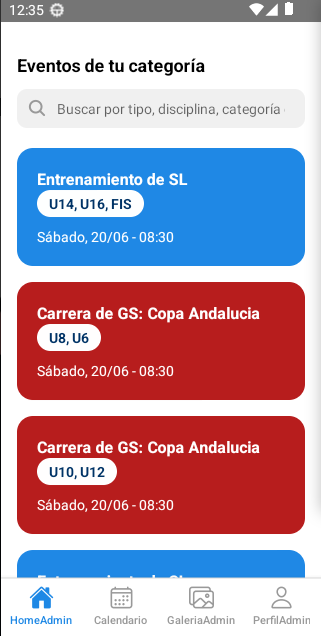
\includegraphics[width=\textwidth]{imagenes/inicio_admin.png}
        \caption{Panel principal de administración.}
        \label{fig:inicioAdminPanel}
    \end{subfigure}
    \caption{Página de inicio del administrador.}
    \label{fig:grupo_inicio_administrador}
\end{figure}

\noindent \textbf{Galería}: El submódulo multimedia para el rol de administración centraliza todo el histórico visual de la temporada en un único punto operativo. A través del panel de control, el usuario puede navegar por las categorías específicas del club o situarse sobre la pestaña General, la cual indexa y agrupa cronológicamente por meses todos aquellos recuerdos e imágenes de interés global para la entidad. Al interactuar con el asistente de subida, la aplicación ofrece un privilegio de asignación flexible exclusivo para este rol; el administrador puede discriminar si el nuevo material fotográfico o de vídeo se vuelca únicamente dentro de la sección de un equipo concreto (mediante la opción de pestaña actual) o si se fuerza su publicación directa en el repositorio general para que sea accesible por todo el cuerpo técnico, compartiendo el resto de funciones de visualización y purga descritas previamente en la Figura~\ref{fig:cuadridula_galeria_multimedia}.

\begin{figure}[htbp]
    \centering
    \begin{subfigure}[t]{0.45\textwidth}
        \centering
        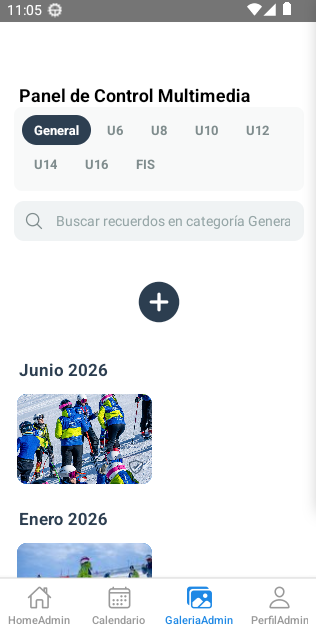
\includegraphics[width=\textwidth]{imagenes/galeria_admin.png}
        \caption{Repositorio en vista General.}
        \label{fig:galeriaAdminGeneral}
    \end{subfigure}
    \hfill
    \begin{subfigure}[t]{0.45\textwidth}
        \centering
        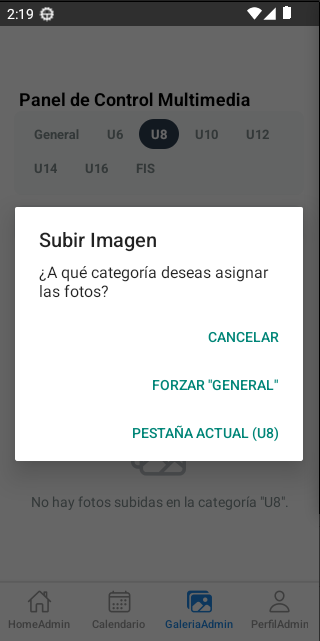
\includegraphics[width=\textwidth]{imagenes/añadir_galeria_admin.png}
        \caption{Selector de asignación multimedia.}
        \label{fig:anadirGaleriaAdmin}
    \end{subfigure}
    \caption{Interfaces del panel de control multimedia del administrador: visualización del repositorio global (a) y asistente de segmentación de cargas (b).}
    \label{fig:modulo_galeria_administracion_completo}
\end{figure}

\noindent \textbf{Perfil de Administración:} La interfaz de perfil del administrador constituye el núcleo de gobernanza y control de toda la plataforma tecnológica.
\newpage
\begin{figure}[htbp]
    \centering
    \begin{subfigure}[t]{0.22\textwidth}
        \centering
        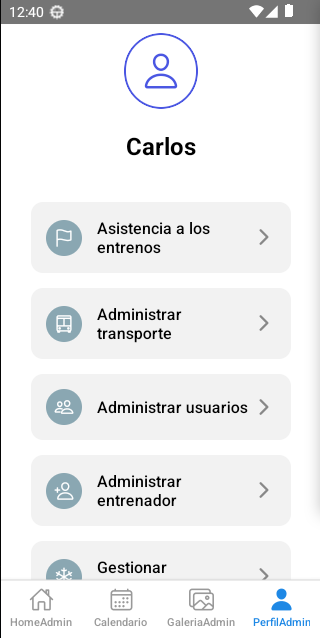
\includegraphics[width=\textwidth]{imagenes/perfil_admin.png}
        \caption{Menú del perfil administrador.}
        \label{fig:perfilAdmin}
    \end{subfigure}
    \hfill
    \begin{subfigure}[t]{0.22\textwidth}
        \centering
        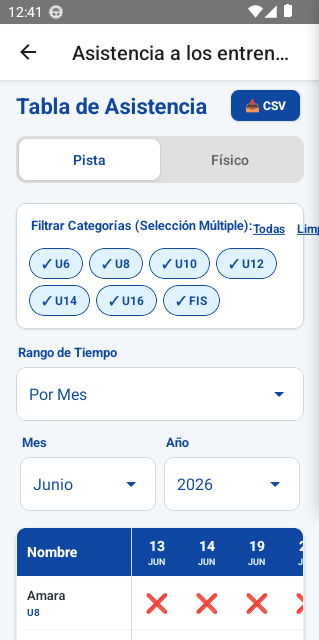
\includegraphics[width=\textwidth]{imagenes/asistencia_pista_admin.png}
        \caption{Tabla de entrenamientos en pista.}
        \label{fig:asistenciaPistaAdmin}
    \end{subfigure}
    \hfill
    \begin{subfigure}[t]{0.22\textwidth}
        \centering
        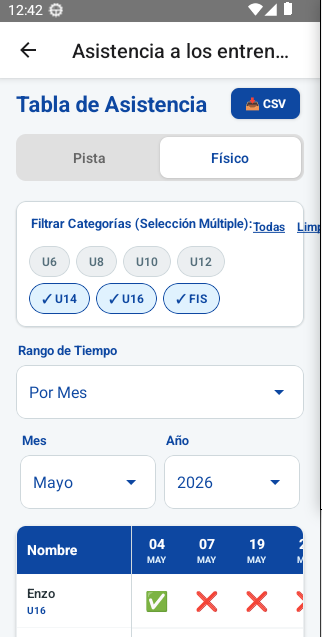
\includegraphics[width=\textwidth]{imagenes/asistencia_entreno_admin.png}
        \caption{Tabla de preparación física.}
        \label{fig:asistenciaEntrenoAdmin}
    \end{subfigure}
    \hfill
    \begin{subfigure}[t]{0.22\textwidth}
        \centering
        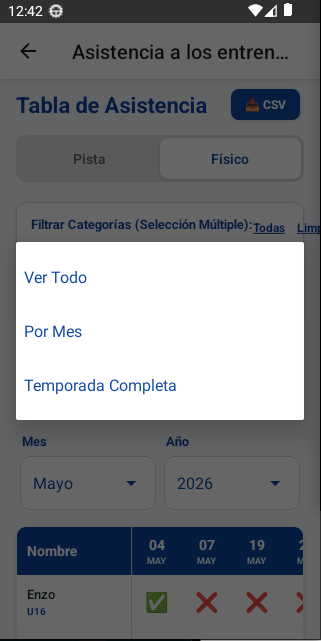
\includegraphics[width=\textwidth]{imagenes/filtro_asistencia.png}
        \caption{Filtro por rangos de tiempo.}
        \label{fig:filtroAsistencia}
    \end{subfigure}
    
    \caption{Módulos de navegación, control de asistencia multicategoría y filtrado temporal avanzado para el rol de administración.}
    \label{fig:suite_administrador_bloque1}
\end{figure}

\begin{figure}[htbp]
    \centering
    \begin{subfigure}[t]{0.22\textwidth}
        \centering
        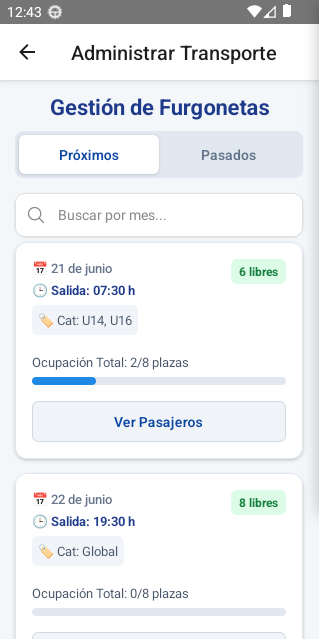
\includegraphics[width=\textwidth]{imagenes/furgo_admin.png}
        \caption{Gestión global de transporte.}
        \label{fig:furgoAdmin}
    \end{subfigure}
    \hfill
    \begin{subfigure}[t]{0.22\textwidth}
        \centering
        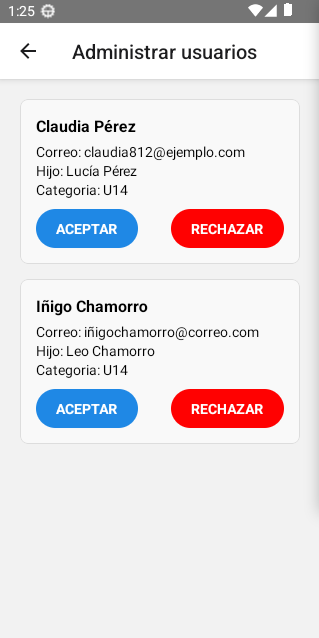
\includegraphics[width=\textwidth]{imagenes/solicitud_usuarios.png}
        \caption{Peticiones de acceso.}
        \label{fig:solicitudUsuarios}
    \end{subfigure}
    \hfill
    \begin{subfigure}[t]{0.22\textwidth}
        \centering
        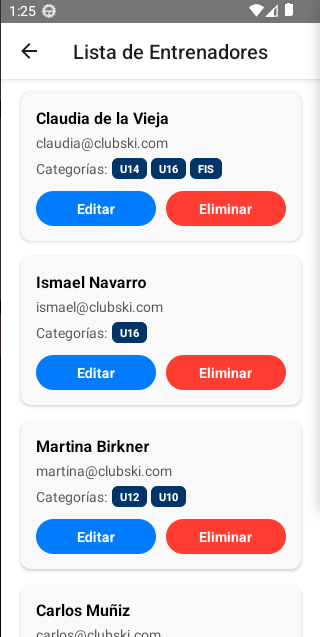
\includegraphics[width=\textwidth]{imagenes/lista_entrenadores.png}
        \caption{Censo de entrenadores.}
        \label{fig:listaEntrenadores}
    \end{subfigure}
    \hfill
    \begin{subfigure}[t]{0.22\textwidth}
        \centering
        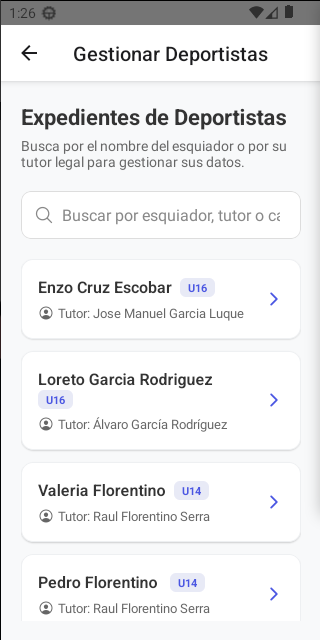
\includegraphics[width=\textwidth]{imagenes/lista_deportistas.png}
        \caption{Expedientes de deportistas.}
        \label{fig:listaDeportistas}
    \end{subfigure}
    
    \caption{Paneles logísticos de transporte, moderación de altas de usuarios y mantenimiento CRUD de los censos del club.}
    \label{fig:suite_administrador_bloque2}
\end{figure}

\noindent \textbf{Panel Central de Configuración Administrativa:} Constituye el punto de partida para las acciones de gobernanza de la plataforma que se muestran visualmente en la Figura~\ref{fig:perfilAdmin}. A diferencia de las vistas simplificadas de otros roles, esta pantalla expone de forma directa la botonera de acceso a todas las funcionalidades críticas de control: auditoría de asistencia, control del transporte, validación de altas de usuarios y mantenimiento del censo de entrenadores y esquiadores del club. \par \smallskip

\noindent \textbf{Asistencia a los entrenamientos:} Este submódulo eleva las capacidades de consulta en comparación con la interfaz técnica básica, tal y como se observa en la Tabla de entrenamientos en pista (Figura~\ref{fig:asistenciaPistaAdmin}) y en la Tabla de preparación física (Figura~\ref{fig:asistenciaEntrenoAdmin}). Permite al administrador monitorizar las asistencias segmentando simultáneamente múltiples categorías mediante un selector de fichas dinámico. El componente añade el menú interactivo de la Figura~\ref{fig:filtroAsistencia} para delimitar el rango de tiempo de la auditoría (pudiendo elegir entre ver todo el histórico, filtrar por mes o evaluar la temporada completa) e integra un botón dedicado para procesar y descargar el histórico consolidado de asistencia en un documento plano con formato CSV. Adicionalmente, el sistema se conecta de forma directa con el visualizador gráfico analizado mediante un componente selector que filtra las métricas y tasas individuales de asistencia de cada corredor. \par \smallskip

\noindent \textbf{Asistencia Transporte:} Interfaz de administración para la flota de furgonetas colectivas de la entidad reflejada en la Figura~\ref{fig:furgoAdmin}. Muestra las rutas programadas ordenadas cronológicamente, pero a diferencia del cuerpo técnico, el administrador cuenta con etiquetas visuales de clasificación que diferencian si el traslado pertenece a categorías combinadas específicas o si se trata de un transporte asignado de carácter global, facilitando la optimización de los vehículos antes de las salidas a la montaña. \par \smallskip

\noindent \textbf{Altas de usuarios:} Bloque operativo destinado a salvaguardar la integridad de los datos en la base de datos MySQL. El administrador actúa como el filtro de seguridad de la plataforma a través de la cola de moderación de la Figura~\ref{fig:solicitudUsuarios} que expone los datos de los nuevos tutores registrados, permitiendo aceptar o rechazar su vinculación al sistema. Asimismo, provee herramientas de mantenimiento CRUD (*Create, Read, Update, Delete*) sobre los expedientes técnicos de los entrenadores en la Figura~\ref{fig:listaEntrenadores} (modificando sus categorías federativas asociadas) y las fichas de los deportistas de la Figura~\ref{fig:listaDeportistas}, donde se indexa el buscador dinámico para rastrear esquiadores y tutores legales de manera integrada.

\subsection{Perfil del Padre / Tutor Legal}
\label{subsec:rol_padre}
El perfil orientado a las familias se enfoca en la transparencia informativa y la conciliación logística.

\noindent \textbf{Inicio y Gestión de Inscripciones:} Constituye el punto de acceso centralizado del rol de tutor legal. El comportamiento del panel principal restringe el flujo de información para que solo aparezcan reflejados aquellos eventos y entrenamientos en los que el padre ha apuntado explícitamente a sus hijos mediante el componente de la Figura~\ref{fig:detalleApuntar}. Al presionar sobre cualquiera de las actividades programadas, el sistema redirige a la vista de detalles, desde donde es posible realizar el seguimiento técnico o desapuntar a los menores de la sesión si surge algún imprevisto logístico. \par \smallskip

\noindent \textbf{Control de Asistencia:} Interfaz dedicada a la edición de la asistencia y la reserva de transporte para cada corredor vinculado al tutor. Como se observa en las Figuras~\ref{fig:detallePadre}, \ref{fig:desapuntarDeportista} y \ref{fig:desapuntarTransporte}, el componente renderiza selectores individuales para cada hijo, indicando mediante iconos visuales si disponen de plaza confirmada en la furgoneta del club. Desde este panel, el tutor puede alternar el conmutador dinámico para solicitar transporte, guardar los cambios en tiempo real o anular la asistencia completa a través del botón de cancelación de inscripción, lo que libera de forma automática el asiento en el vehículo y actualiza el censo del entrenamiento en el servidor. \par \smallskip

\noindent \textbf{Galería:} Módulo de consulta visual diseñado bajo estrictas políticas de privacidad de los deportistas menores de edad. A diferencia del panel general de administración, en esta pantalla únicamente se exponen las pestañas correspondientes a las categorías deportivas a las que pertenecen los hijos del usuario (como la pestaña U14 activa en la Figura~\ref{fig:galeriaPadre}). El backend discrimina las peticiones web de imágenes para que el tutor solo visualice el repositorio fotográfico y de vídeo de dichos niveles; asimismo, al interactuar con el carrete mediante el menú contextual de la Figura~\ref{fig:descargarPadre}, se habilita la descarga local en el almacenamiento del dispositivo móvil.

\begin{figure}[htbp]
    \centering
    \begin{subfigure}[t]{0.28\textwidth}
        \centering
        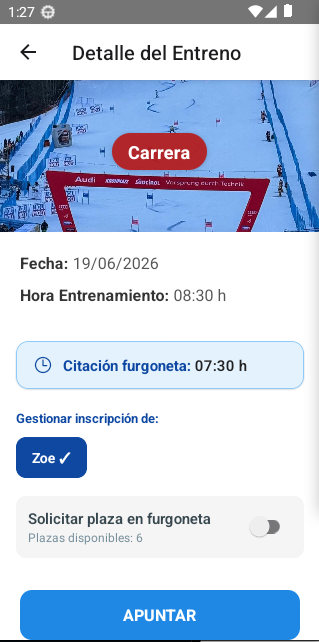
\includegraphics[width=\textwidth]{imagenes/detalle_apuntar.png}
        \caption{Inscripción de deportistas.}
        \label{fig:detalleApuntar}
    \end{subfigure}
    \hfill
    \begin{subfigure}[t]{0.28\textwidth}
        \centering
        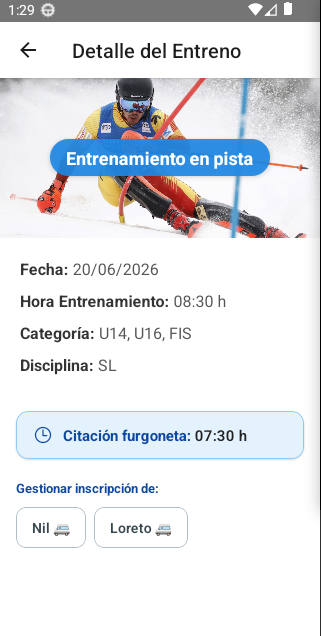
\includegraphics[width=\textwidth]{imagenes/detalle_padre.png}
        \caption{Detalle del entrenamiento.}
        \label{fig:detallePadre}
    \end{subfigure}
    \hfill
    \begin{subfigure}[t]{0.28\textwidth}
        \centering
        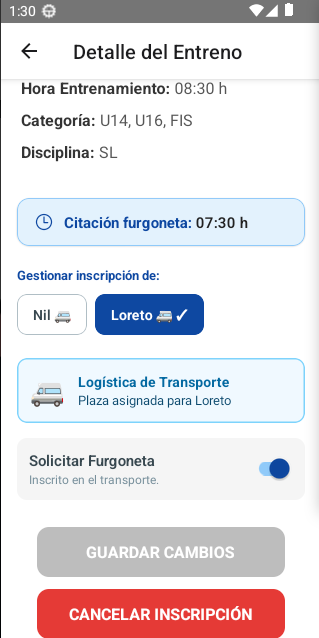
\includegraphics[width=\textwidth]{imagenes/desapuntar_deportista.png}
        \caption{Gestión e inscripción de transporte.}
        \label{fig:desapuntarDeportista}
    \end{subfigure}
    
    \caption{Flujo inicial operativo del rol de tutor: inscripción a sesiones del club (a), consulta del estado técnico de la actividad (b) y reserva de plaza en transporte colectivo (c).}
    \label{fig:suite_padre_fase1}
\end{figure}

\begin{figure}[htbp]
    \centering
    \begin{subfigure}[t]{0.28\textwidth}
        \centering
        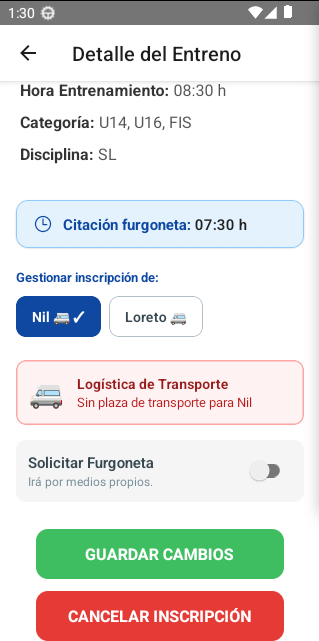
\includegraphics[width=\textwidth]{imagenes/desapuntar_transporte.png}
        \caption{Modificación de preferencias logísticas.}
        \label{fig:desapuntarTransporte}
    \end{subfigure}
    \hfill
    \begin{subfigure}[t]{0.28\textwidth}
        \centering
        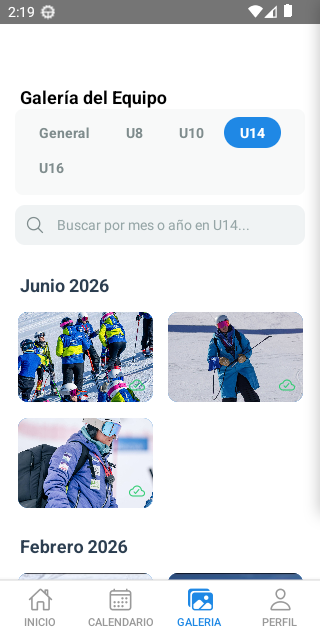
\includegraphics[width=\textwidth]{imagenes/galeria_padre.png}
        \caption{Repositorio multimedia segmentado.}
        \label{fig:galeriaPadre}
    \end{subfigure}
    \hfill
    \begin{subfigure}[t]{0.28\textwidth}
        \centering
        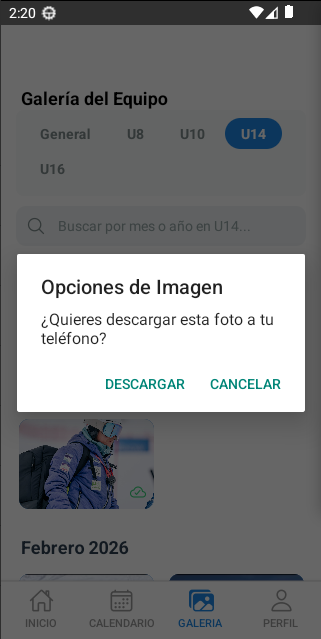
\includegraphics[width=\textwidth]{imagenes/descargar_padre.png}
        \caption{Confirmación de descarga local.}
        \label{fig:descargarPadre}
    \end{subfigure}
    
    \caption{Flujo de edición y consulta multimedia: alteración de traslados a medios propios (a), visualización de carrete restringido (b) y almacenamiento de capturas (c).}
    \label{fig:suite_padre_fase2}
\end{figure}

\newpage
\noindent \textbf{Perfil del Tutor:} Representa el centro de configuración y navegación para el rol de tutor legal que se ilustra en la Figura~\ref{fig:perfilPadreMenu}. \par \smallskip

\noindent \textbf{Análisis Estadístico de Asistencia:} Interfaz analítica encargada de evaluar la constancia deportiva de los corredores mediante la integración de la librería \texttt{react-native-chart-kit}. Como se detalla en las Figuras~\ref{fig:asistenciaPadrePista}, \ref{fig:pickerAsistenciaPadre} y \ref{fig:asistenciaPadreFisico}, el sistema incorpora un componente modal de selección que extrae exclusivamente los nombres de los hijos del usuario. Al seleccionar un atleta y delimitar el mes o año de consulta, el componente renderiza un gráfico circular (*PieChart*) reflectante del porcentaje de asistencia del menor, discriminando dinámicamente mediante pestañas interactivas entre las sesiones técnicas en nieve (pista) y la preparación física. \par \smallskip

\noindent \textbf{Supervisión del Histórico de Furgoneta:} Módulo informativo dedicado al control de la logística del club que se expone en las Figuras~\ref{fig:transportePadreProximos} y \ref{fig:transportePadreHistorial}. Dispone de un sistema bimodal segmentado entre las rutas programadas para los días venideros (próximos) y el registro retrospectivo de trayectos completados (historial), mostrando los deportistas apuntados parametrizados por colores que informan al tutor si sus hijos tienen la plaza confirmada o cancelada para cada fecha determinada. \par \smallskip

\noindent \textbf{Administración del Censo Familiar y Altas:} Bloque operativo orientado a la autogestión de los expedientes de los menores asociados a la cuenta del tutor legal. Reflejado en las Figuras~\ref{fig:administrarDeportistasPadre} y \ref{fig:anadirHijoForm}.

\begin{figure}[htbp]
    \centering
    \begin{subfigure}[t]{0.20\textwidth}
        \centering
        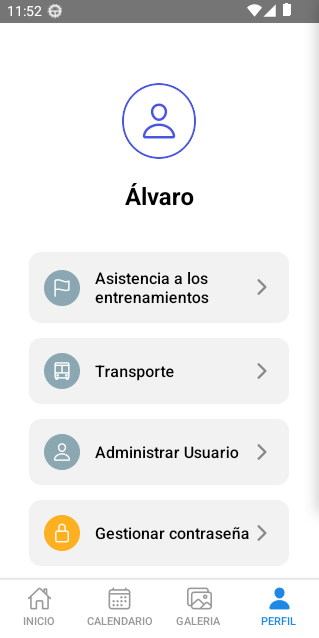
\includegraphics[width=\textwidth]{imagenes/perfil_padre.png}
        \caption{Menú del perfil del padre.}
        \label{fig:perfilPadreMenu}
    \end{subfigure}
    \hfill
    \begin{subfigure}[t]{0.20\textwidth}
        \centering
        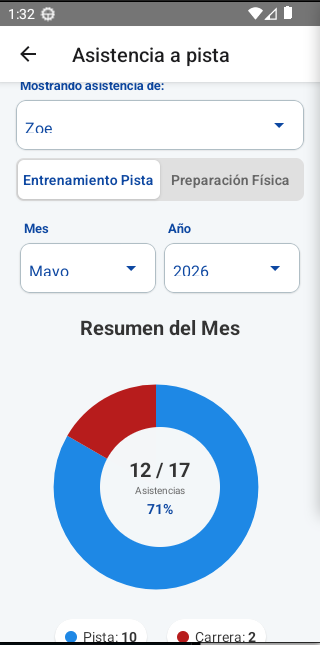
\includegraphics[width=\textwidth]{imagenes/asistencia_padre.png}
        \caption{Métricas de asistencia en pista.}
        \label{fig:asistenciaPadrePista}
    \end{subfigure}
    \hfill
    \begin{subfigure}[t]{0.20\textwidth}
        \centering
        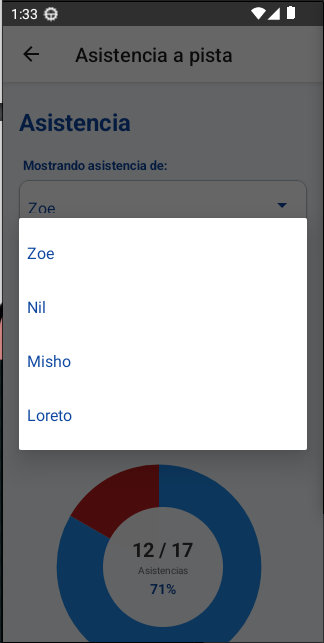
\includegraphics[width=\textwidth]{imagenes/picker_asistencia.png}
        \caption{Selector dinámico de deportista.}
        \label{fig:pickerAsistenciaPadre}
    \end{subfigure}
    \hfill
    \begin{subfigure}[t]{0.20\textwidth}
        \centering
        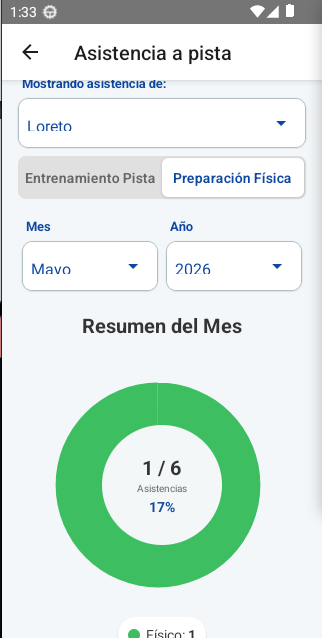
\includegraphics[width=\textwidth]{imagenes/asistencia_fisico_padre.png}
        \caption{Métricas de preparación física.}
        \label{fig:asistenciaPadreFisico}
    \end{subfigure}
    
    \caption{Paneles del rol de tutor: menú de configuración (a), gráficas estadísticas de asistencia (b, d) y componente de selección filial (c).}
    \label{fig:suite_perfil_padre_bloque1}
\end{figure}

\begin{figure}[htbp]
    \centering
    \begin{subfigure}[t]{0.20\textwidth}
        \centering
        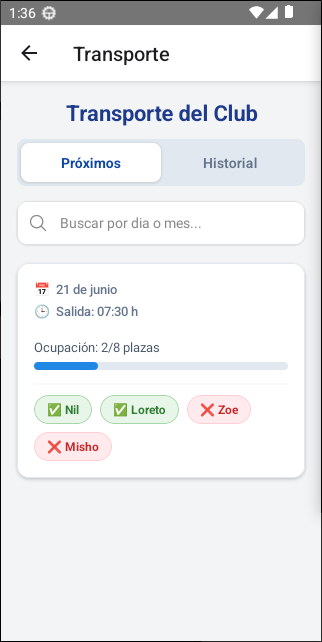
\includegraphics[width=\textwidth]{imagenes/transporte_padre.png}
        \caption{Estado de rutas próximas.}
        \label{fig:transportePadreProximos}
    \end{subfigure}
    \hfill
    \begin{subfigure}[t]{0.20\textwidth}
        \centering
        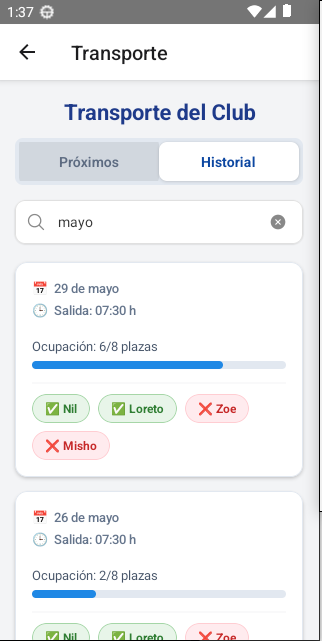
\includegraphics[width=\textwidth]{imagenes/transporte_historial.png}
        \caption{Historial logístico de traslados.}
        \label{fig:transportePadreHistorial}
    \end{subfigure}
    \hfill
    \begin{subfigure}[t]{0.20\textwidth}
        \centering
        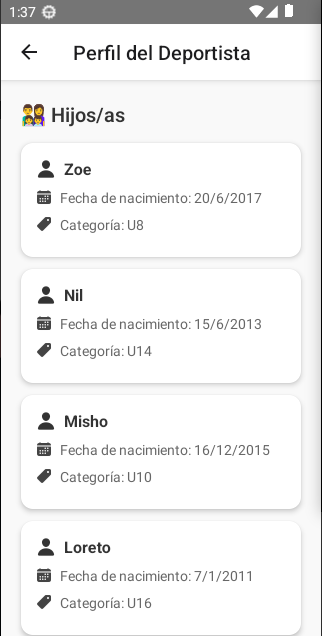
\includegraphics[width=\textwidth]{imagenes/administrar_deportistas_padre.png}
        \caption{Censo de hijos vinculados.}
        \label{fig:administrarDeportistasPadre}
    \end{subfigure}
    \hfill
    \begin{subfigure}[t]{0.20\textwidth}
        \centering
        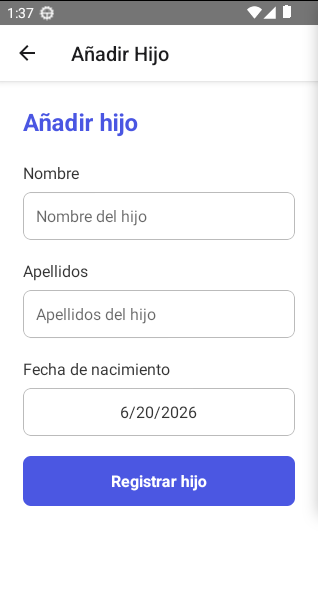
\includegraphics[width=\textwidth]{imagenes/añadir_hijo.png}
        \caption{Formulario de registro de menor.}
        \label{fig:anadirHijoForm}
    \end{subfigure}
    
    \caption{Módulos de supervisión de transporte colectivo (a, b) y herramientas de gestión del censo familiar en la plataforma (c, d).}
    \label{fig:suite_perfil_padre_bloque2}
\end{figure}

